\documentclass{mimore}

\newcommand{\sAuthor  }{Dave Mannion}
\newcommand{\sTitle   }{Gene Family Prediction \& ML}
\newcommand{\sSubtitle}{Machine Learning and DNA Sequence Classification}
\newcommand{\sSubject }{Bootcamp Capstone Report}
\newcommand{\sCourse  }{UCSD Machine Learning \& Engineering}
\newcommand{\sDate    }{\today}

\bibliography{Capstone}

%%%%%%%%%%%%%%%%%%%%%%%%%%%%%%%%%%%%%%%%%%%%%%%%%%%%%%%%%%%%%%%%%%%%%%%%
% TikZ & pgfplots
%%%%%%%%%%%%%%%%%%%%%%%%%%%%%%%%%%%%%%%%%%%%%%%%%%%%%%%%%%%%%%%%%%%%%%%%

\usepackage{tikz}
\usepackage{pgfplots}
\usepackage{minted}
\pgfplotsset{compat=1.12}

% Permits accessing the smallest and largest x value of a plot
\makeatletter
  \newcommand{\pgfplotsxmin}{\pgfplots@xmin}
  \newcommand{\pgfplotsxmax}{\pgfplots@xmax}
\makeatother

% Permits accessing the smallest and largest y value of a plot
\makeatletter
  \newcommand{\pgfplotsymin}{\pgfplots@ymin}
  \newcommand{\pgfplotsymax}{\pgfplots@ymax}
\makeatother

%%%%%%%%%%%%%%%%%%%%%%%%%%%%%%%%%%%%%%%%%%%%%%%%%%%%%%%%%%%%%%%%%%%%%%%%
% Begin of main document
%%%%%%%%%%%%%%%%%%%%%%%%%%%%%%%%%%%%%%%%%%%%%%%%%%%%%%%%%%%%%%%%%%%%%%%%

\begin{document}

  \maketitle

  \tableofcontents
  \bookmarksetup{startatroot}

  %%%%%%%%%%%%%%%%%%%%%%%%%%%%%%%%%%%%%%%%%%%%%%%%%%%%%%%%%%%%%%%%%%%%%%
  % Add your sources here. You may also directly input LaTeX commands
  % here, but the use of `\include` is strongly encouraged.
  %%%%%%%%%%%%%%%%%%%%%%%%%%%%%%%%%%%%%%%%%%%%%%%%%%%%%%%%%%%%%%%%%%%%%%

  \section{Introduction}

\begin{table}[tb]
  \centering
  \begin{tabular}{lSS}
    \toprule
    \textbf{Gene Family}      & \textbf{Count} & \textbf{Class Label}\\
    \midrule
    G protein coupled receptors	 & 531 & 1\\
    Tyrosine kinase	 & 534	 & 2\\
    Tyrosine phospotase	 & 349	 & 3\\
    Synthetase	 & 632	 & 4\\
    Synthase	 & 711	 & 5\\
    Ion channel	 & 240	 & 6\\
    Transcription factor	 & 1341	 & 7\\
    \bottomrule
  \end{tabular}
  \caption{
    Gene Families represented by Human DNA coding sequences.
  }
  \label{tab:GeneFamilies}
\end{table}

Here we examine NLP algorithms to develop a Machine Learning model for making predictions on sequences of Nucleic Acid text. Specifically, we train a Multinomial Na\"ive Bayes classifier on Human DNA Coding Sequences to predict Gene Families. In addition to Human sequences, predictive testing was also performed on Chimpanzee and Dog DNA coding sequences.
%
\autoref{tab:GeneFamilies} above shows Gene Families in the dataset.

\subsection{Motivation}

This Capstone project was selected to provide an opportunity to explore the application of NLP methods to biological text-based sequence data.


\subsection{Exploratory Work}

Prior to selecting this Capstone project, recent work in ML applied to biological sequences was surveyed in order to identify the feasability and scope of a project appropriate for this course.  Method feasability focused on LDA, NB and LSTM models. Some of this work is linked to Jupyter notebooks or original papers and includes protein classification\footnote{\url{https://github.com/ai-dave/ml-gene-pub/blob/main/protein-classification.ipynb}},
Sapien/Neandertal sequence classification\footnote{\url{https://github.com/ai-dave/ml-gene-pub/blob/main/Deep_Learning_on_Ancient_DNA.ipynb}},
Neandertal DNA introgression\footnote{\url{https://github.com/ai-dave/ml-gene-pub/blob/main/Deep_Learning_Neanderthal_Introgression.ipynb}}, 
CRISPR gRNA design tools\footnote{\url{https://pubmed.ncbi.nlm.nih.gov/31533522/}},
Bacterial Classification with RNNs\footnote{\url{https://github.com/lelugom/wgs_classifier}}, 
Bacteria taxonomic classification\footnote{\url{https://www.researchgate.net/publication/348432006_Bacteria_taxonomic_classification_using_Machine_learning_models}},
Ribosmal RNA analysis\footnote{\url{https://github.com/ai-dave/ml-gene-pub/blob/main/gnb-rdp.ipynb}}\textsuperscript{,}\footnote{\url{https://github.com/ai-dave/ml-gene-pub/blob/main/lda-compare-silva.ipynb}}\textsuperscript{,}\footnote{\url{https://github.com/ai-dave/ml-gene-pub/blob/main/lda-rdp.ipynb}}\textsuperscript{,}\footnote{\url{https://github.com/ai-dave/ml-gene-pub/blob/main/lstm-random-noise.ipynb}}\textsuperscript{,}\footnote{\url{https://github.com/ai-dave/ml-gene-pub/blob/main/lstm-rdp.ipynb}},
Viral and Single-celled Eukaryote Taxonomy classification\footnote{\url{https://github.com/ai-dave/ml-gene-pub/blob/main/ncbi_lstm_poc.ipynb}}\textsuperscript{,}\footnote{\url{https://github.com/ai-dave/ml-gene-pub/blob/main/Eukaryota-Amoebozoa-Discosea.ipynb}},
Wolf/Dhole classification\footnote{\url{https://github.com/ai-dave/ml-gene-pub/blob/main/Dhole-Wolfe-LDA.ipynb}}\textsuperscript{,}\footnote{\url{https://github.com/ai-dave/ml-gene-pub/blob/main/Dhole-Wolfe-LSTM.ipynb}}\textsuperscript{,}\footnote{\url{https://github.com/ai-dave/ml-gene-pub/blob/main/Dhole-Wolfe.ipynb}}.

\subsection{Capstone Project Work}
Jupyter notebook for the Capstone Project is is available from a github repo\footnote{\url{https://github.com/ai-dave/ml-gene-pub/blob/main/gene-family-human-chimp-dog.ipynb}}.
%  \section{Data}

\subsection{Source}

The data for this project came from a Kaggle notebook, DNA Sequencing with Machine Learning\footnote{\url{https://www.kaggle.com/code/nageshsingh/demystify-dna-sequencing-with-machine-learning/data}}.

\subsection{Labeling}


\subsection{Preprocessing: K-Mer vectorization}


\subsection{Feature Extraction/Embedding}

Use CountVectorizer to convert k-merized sequences to a matrix of token counts\footnote{\url{https://scikit-learn.org/stable/modules/generated/sklearn.feature_extraction.text.CountVectorizer.html}}.

\subsection{Model Building}

\subsection{Model Performance}

\subsection{Model Deployment}


  \section{Data}
%
  \begin{figure}
    \centering
    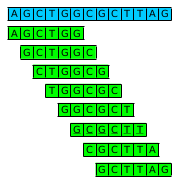
\includegraphics[scale=1]{kmers}
    \caption{%
      6-mer \textit{"word"} production from original sequence.
    }
    \label{fig:kmers}
  \end{figure}
%
\subsection{Source}

The data for this project came from a Kaggle notebook, \textit{DNA Sequencing with Machine Learning}\footnote{\url{https://www.kaggle.com/code/nageshsingh/demystify-dna-sequencing-with-machine-learning/data}}.
%
DNA Coding Sequences are mostly comprised of exons and, in this corpus, range in length from  $\sim$1000 to $\sim$3,500 bases.

\subsection{Labeling}
Each sequence in the corpus of sequence data was annotated with one of seven Gene Families.  The Gene Family annotation was translated into an integer class label \textit{c} in $\{1, 2, 3, 4, 5, 6, 7\}$


\subsection{Preprocessing: K-mer vectorization}
%
The nucleotide bases comprise an \textit{alphabet} of the four letters \textit{b} in $\{A, G, C, T\}$.  A \textit{K-mer} is a \textit{k}-letter word comprised from \textit{letters} of this \textit{alphabet}.  Here we let \textit{k=6}.  The \textit{dictionary} contains up to $4^{6}$ \textit{words}, each 6 letters in length.\footnote{Dictionary size calculated as $alphabetSize^{wordLength}$ $\Rightarrow$ $4^{6}$ $\Rightarrow$ 4,096 words.}

\autoref{fig:kmers} above depicts 6bp \textit{"words"} derived from a sequence of the original corpus.  From this point on, all vectorization is based on a corpus of \textit{6-mer "words"} rather than the original sequences.
%

  \section{Feature Engineering}
%
  \begin{figure}
    \centering
    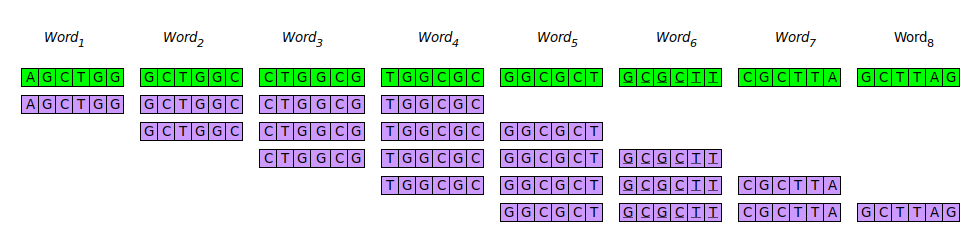
\includegraphics[scale=0.4]{ngrams}
    \caption{%
       4-word n-gram (\textit{4-gram}) phrases generated from 6-mer words representing the original nucleic acid sequence.
    }
    \label{fig:ngrams}
  \end{figure}
%
  \begin{figure}
    \centering
    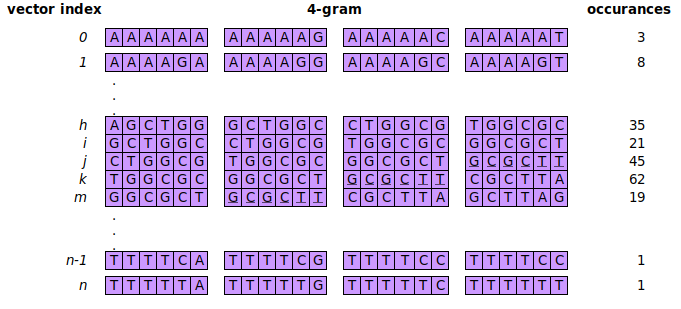
\includegraphics[scale=0.4]{count_vector}
    \caption{%
       4-word n-gram (\textit{4-gram}) phrases generated from 6-mer words representing the original nucleic acid sequence.
    }
    \label{fig:count-vector}
  \end{figure}
%

After converting contiguous nucleotide sequences into 6-mer words, \textit{Bag of Words} model was used to produce document vectors.


\subsection{n-grams}

We use CountVectorizer\footnote{\url{https://scikit-learn.org/stable/modules/generated/sklearn.feature_extraction.text.CountVectorizer.html}} to convert k-merized sequences to a matrix of token counts.

\autoref{fig:ngrams} above shows 4-gram phrases generated from a series of 6-mers of the original sequence. 
%
\subsection{Frequency Vectorization}
The frequencies of ordered 4-grams from each single nucleic acid k-merized sequence will produce a histogram based on the occurance of the 4-gram.
\autoref{fig:count-vector} above shows a Count Vector formed from 4-gram frequencies. 
%

  \section{Modeling}
%
\begin{table}[tb]
  \centering
  \begin{tabular}[t]{lSSSSSSSSS}
    \toprule
%    \textbf{Predicted} 
    \begin{tabular}[l]{@{}c@{}}\textbf{Predicted}\\ \textbf{Actual}\end{tabular}
    & \textbf{1}  & \textbf{2}  & \textbf{3}  & \textbf{4}  & \textbf{5}  & \textbf{6} & \textbf{7}\\

    \midrule
    1 & 113 &  0 &  0 &   0 &   1 &  0 &   10\\
    2 &   0 & 82 &  0 &   0 &   0 &  0 &   3\\
    3 &   0 &  0 & 65 &   0 &   0 &  0 &   4\\
    4 &   0 &  0 &  0 & 125 &   2 &  0 &   1\\
    5 &   3 &  0 &  0 &   0 & 121 &  0 &   0\\
    6 &   1 &  0 &  0 &   0 &   0 & 38 &   0\\
    7 &   1 &  0 &  0 &   0 &   1 &  0 & 233\\
    \bottomrule
  \end{tabular}
  \caption{
    Confusion matrix for predictions on human test DNA sequence.
  }
  \label{tab:confusion-human}
\end{table}
%
%
\begin{table}[tb]
  \centering
  \begin{tabular}{lSS}
    \toprule
    \midrule
	accuracy & 0.966\\
	precision & 0.968\\
	recall & 0.966\\
	f1 & 0.966\\
    \bottomrule
  \end{tabular}
  \caption{
    Accuracy, precision, recall
  }
  \label{tab:confusion-human-summary}
\end{table}
%


\subsection{Training}
We are building a Multinomial Naive Bayes classifier model using  \textit{MultinomialNB}\footnote{\url{https://scikit-learn.org/stable/modules/generated/sklearn.naive_bayes.MultinomialNB.html}} and training it on Human DNA sequences \textit{k-merized} and embedded as 4-gram frequency histogram vectors:
\begin{minted}{python}
X_train, X_test, y_train, y_test = train_test_split(X, y_human, test_size=0.2, random_state=42)

classifier = MultinomialNB(alpha=0.1)
classifier.fit(X_train, y_train)
pickle.dump(classifier, open('model-human.pkl','wb'))
\end{minted}
%
\subsection{Performance}
\autoref{tab:confusion-human} and \autoref{tab:confusion-human-summary} above show Confusion Matrix and accuracy/precision/recall values on the Test set of Human DNA.

  \section{Results: Chimpanzee DNA}

\autoref{tab:confusion-chimpanzee} and \autoref{tab:confusion-chimpanzee-summary} above show results of testing chimpanzee DNA Coding sequences against a model trained on Human DNA for the seven Gene Families:
%
\begin{table}[tb]
  \centering
  \begin{tabular}[t]{lSSSSSSSSS}
    \toprule
%    \textbf{Predicted} 
    \begin{tabular}[l]{@{}c@{}}\textbf{Predicted}\\ \textbf{Actual}\end{tabular}
    & \textbf{1}  & \textbf{2}  & \textbf{3}  & \textbf{4}  & \textbf{5}  & \textbf{6} & \textbf{7}\\

    \midrule
    1 & 224 &   0 &   0 &   0 &   3 &   0 &   6\\
    2 &   0 & 182 &   0 &   0 &   0 &   0 &   3\\
    3 &   0 &   0 & 137 &   0 &   0 &   0 &   7\\
    4 &   0 &   0 &   0 & 222 &   3 &   0 &   7\\
    5 &   2 &   0 &   0 &   0 & 259 &   0 &   0\\
    6 &   1 &   0 &   0 &   0 &   0 & 108 &   0\\
    7 &   0 &   0 &   0 &   0 &   1 &   0 & 521\\
    \bottomrule
  \end{tabular}
  \caption{
    Confusion matrix for predictions on chimpanzee DNA sequences.
  }
  \label{tab:confusion-chimpanzee}
\end{table}
%
%
\begin{table}[tb]
  \centering
  \begin{tabular}{lSS}
    \toprule
    \midrule
	accuracy & 0.984\\
	precision & 0.984\\
	recall & 0.984\\
	f1 & 0.984\\
    \bottomrule
  \end{tabular}
  \caption{
    Accuracy, precision, recall
  }
  \label{tab:confusion-chimpanzee-summary}
\end{table}
%

  \section{Results: Dog DNA}

\autoref{tab:confusion-dog} and \autoref{tab:confusion-dog-summary} above show results of testing dog DNA Coding sequences against a model trained on Human DNA for the seven Gene Families.
%
\begin{table}[tb]
  \centering
  \begin{tabular}[t]{lSSSSSSSSS}
    \toprule
%    \textbf{Predicted} 
    \begin{tabular}[l]{@{}c@{}}\textbf{Predicted}\\ \textbf{Actual}\end{tabular}
    & \textbf{1}  & \textbf{2}  & \textbf{3}  & \textbf{4}  & \textbf{5}  & \textbf{6} & \textbf{7}\\

    \midrule
    1 & 119 &   0 &   0 &   0 &   1 &   0 &   7\\
    2 &   0 &  60 &   0 &   0 &   0 &   0 &  14\\
    3 &   0 &   0 &  45 &   0 &   1 &   0 &  16\\
    4 &   0 &   0 &   0 &  77 &   2 &   0 &  16\\
    5 &   6 &   0 &   0 &   1 & 117 &   0 &   7\\
    6 &   3 &   0 &   0 &   0 &   1 &  51 &   5\\
    7 &   0 &   0 &   0 &   0 &   0 &   0 & 254\\
    \bottomrule
  \end{tabular}
  \caption{
    Confusion matrix for predictions on dog DNA sequences.
  }
  \label{tab:confusion-dog}
\end{table}
%
%
\begin{table}[tb]
  \centering
  \begin{tabular}{lSS}
    \toprule
    \midrule
	accuracy & 0.900\\
	precision & 0.916\\
	recall & 0.900\\
	f1 & 0.900\\
    \bottomrule
  \end{tabular}
  \caption{
    Accuracy, precision, recall
  }
  \label{tab:confusion-dog-summary}
\end{table}
%

  \section{Deployment}

\subsection{Architecture}
\begin{itemize}
  \item Server HTTP framework: Flask
  \item Deployed platform: Docker
\end{itemize}


\subsection{Resources}

\begin{itemize}
  \item Deploy from: \url{https://github.com/ai-dave/capstone/tree/main/deploy} 
  \item Deployed model: \url{http://45.33.108.171/home}
\end{itemize}

  \section{Resources}



%%%%%%%%%%%%%%%%%%%%%%%%%%%%%%%%%%%%%%%%%%%%%%%%%%%%%%%%%%%%%%%%%%%%%%%%
% Back matter: don't change anything here
%%%%%%%%%%%%%%%%%%%%%%%%%%%%%%%%%%%%%%%%%%%%%%%%%%%%%%%%%%%%%%%%%%%%%%%%

  \bookmarksetup{startatroot}
  \printbibliography
	
\end{document}
